\documentclass[12pt,a4paper]{report}

% =========================================================================
%                         1. PACKAGES & SETUP
% =========================================================================
\usepackage{lmodern}
\usepackage[utf8]{inputenc}
\usepackage[T1]{fontenc}
\usepackage[english]{babel}
\usepackage[disable]{microtype}
\usepackage{geometry}
\usepackage{graphicx}
\usepackage{xcolor}
\usepackage{titlesec}
\usepackage{eso-pic}
\usepackage{float}
\usepackage{subcaption}
\usepackage{url}
\usepackage{hyperref}
\usepackage{booktabs}
\usepackage{longtable}
\usepackage{array}
\usepackage{multirow}
\usepackage{enumitem}
\usepackage{amsmath}
\usepackage{amssymb}
\usepackage{tikz}
\usepackage{pgfplots}
\usepackage{listings}
\usepackage{algorithm}
\usepackage{algpseudocode}
\usepackage{caption}
\usepackage{fancyhdr}
\usepackage{setspace}

% Geometry settings (must be in preamble)
\geometry{top=2.5cm, bottom=2.5cm, left=2.5cm, right=2.5cm}
\setlength{\emergencystretch}{3em}

% Set header height for fancyhdr compatibility
\setlength{\headheight}{15pt}

% TikZ Libraries for Diagrams
\usetikzlibrary{shapes.geometric, arrows, positioning, fit, backgrounds, calc, shadows}

% PGFPlots settings
\pgfplotsset{compat=1.18}

% Hyperref settings
\hypersetup{
    colorlinks=true,
    linkcolor=blue!60!black,
    citecolor=green!50!black,
    urlcolor=blue!70!black
}

% Code listing style
\lstset{
    basicstyle=\ttfamily\small,
    backgroundcolor=\color{gray!10},
    frame=single,
    breaklines=true,
    numbers=left,
    numberstyle=\tiny\color{gray},
    keywordstyle=\color{blue},
    commentstyle=\color{green!50!black},
    stringstyle=\color{red!70!black}
}

% Define colors for diagrams
\definecolor{primaryblue}{RGB}{41, 128, 185}
\definecolor{secondarygreen}{RGB}{39, 174, 96}
\definecolor{accentorange}{RGB}{230, 126, 34}
\definecolor{alertred}{RGB}{231, 76, 60}
\definecolor{lightgray}{RGB}{236, 240, 241}

% =========================================================================
%                  2. CUSTOM COMMANDS
% =========================================================================

\newcommand{\titre}[1]{\def\thetitle{#1}}
\newcommand{\UE}[1]{\def\theue{#1}}
\newcommand{\sujet}[1]{\def\thesujet{#1}}
\newcommand{\enseignant}[1]{\def\theenseignant{#1}}
\newcommand{\eleves}[1]{\def\theeleves{#1}}
\newcommand{\jury}[1]{\def\thejury{#1}}

\newcommand{\fairepagedegarde}{
    \begin{titlepage}
        \thispagestyle{empty}
        \centering
        
        % School Logo
        \vspace*{0.5cm}
        \includegraphics[width=0.5\textwidth]{images/ensam_logo.png}
        
        \vspace{0.5cm}
        
        {\scshape\LARGE \theue \par}
        \vspace{0.3cm}
        {\scshape\Large \thesujet \par}
        
        \vspace{2cm}
        
        \rule{\linewidth}{0.5mm} \\[0.4cm]
        {\huge\bfseries \thetitle \par}
        \rule{\linewidth}{0.5mm} \\[1.5cm]
        
        \vspace{2cm}
        
        \begin{minipage}{0.45\textwidth}
            \begin{flushleft} \large
                \emph{Author:}\\
                \theeleves
            \end{flushleft}
        \end{minipage}
        \hfill
        \begin{minipage}{0.45\textwidth}
            \begin{flushright} \large
                \emph{Supervisors:} \\
                \theenseignant
            \end{flushright}
        \end{minipage}

        \vfill
        
        {\large Academic Year 2025-2026\par} 
    \end{titlepage}
}

% Chapter styling
\titleformat{\chapter}[display]
  {\normalfont\bfseries\LARGE}
  {\mdseries\fontsize{50pt}{60pt}\selectfont\chaptertitlename\ \thechapter}
  {20pt}
  {}

\titleformat{name=\chapter,numberless}
  {\normalfont\bfseries\LARGE} 
  {}{0pt}
  {}

% Header/Footer Configuration
\fancyhf{}
\fancyhead[L]{\textit{RadiKal XAI Quality Control System}}
\fancyhead[R]{\thepage}
\fancyfoot[C]{\small Explainable AI for Radiographic Weld Defect Detection}
\renewcommand{\headrulewidth}{0.5pt}
\renewcommand{\footrulewidth}{0.5pt}

% Widow and Orphan control
\widowpenalty=300
\clubpenalty=300
\displaywidowpenalty=300

% =========================================================================
%                             3. DOCUMENT START
% =========================================================================
\begin{document}

% --- Define Report Info ---
\titre{RadiKal: Explainable AI (XAI) for Visual Quality Control\\[0.3cm] Detection and Operator Decision Support\\[0.2cm]\large A Full ERP Solution}
\UE{Higher National School of Arts And Crafts -- Meknes}
\sujet{Expertise Project}
\enseignant{M. T. Masrour \\ Mme. I. Elhassani}
\eleves{Amine EL-HEND}
\jury{}

% --- Title Page ---
\fairepagedegarde
\clearpage

% =========================================================================
%                          PRELIMINARY PAGES
% =========================================================================
\pagenumbering{roman} 
\setcounter{page}{1}
\pagestyle{fancy}

% --- Dedication ---
\cleardoublepage
\thispagestyle{empty}
\vspace*{4cm}
\begin{center} \textbf{\Huge Dedication} \end{center}
\vspace{2cm}
\begin{center} \Large\itshape
To my beloved family, whose unwavering support and encouragement\\
have been the foundation of my academic journey.\\[1cm]
To my professors and mentors at ENSAM Meknes,\\
who have guided me toward excellence in engineering.\\[1cm]
To the industrial quality control professionals worldwide,\\
who strive for perfection in manufacturing safety.
\end{center}

% --- Acknowledgements ---
\newpage
\thispagestyle{empty}
\vspace*{3cm}
\begin{center} \textbf{\Huge Acknowledgements} \end{center}
\vspace{1.5cm}
\begin{center} \large
\begin{minipage}{0.85\textwidth}
I would like to express my sincere gratitude to my supervisors, \textbf{M. T. Masrour} and \textbf{Mme. I. Elhassani}, for their invaluable guidance, continuous support, and expert insights throughout this project. Their mentorship has been instrumental in shaping this research.

\vspace{0.8cm}

I extend my appreciation to the \textbf{Higher National School of Arts and Crafts (ENSAM) Meknes} for providing the academic environment and resources necessary for this work.

\vspace{0.8cm}

Special thanks to the research community behind the \textbf{RIAWELC dataset} and the developers of open-source deep learning frameworks, whose contributions have enabled this research.

\vspace{0.8cm}

Finally, I thank my family and friends for their patience, understanding, and moral support during the demanding phases of this project.
\end{minipage}
\end{center}

% --- Abstract ---
\chapter*{Abstract}
\addcontentsline{toc}{chapter}{Abstract}

Radiographic inspection is a critical non-destructive testing (NDT) method for ensuring the structural integrity of welded joints in industries such as aerospace, nuclear, and oil \& gas. Traditional manual inspection is time-consuming, subjective, and prone to human error. This project presents \textbf{RadiKal}, an Explainable Artificial Intelligence (XAI) system designed for automated visual quality control of radiographic weld images.

RadiKal integrates modern, high-performance deep learning models---specifically \textbf{YOLOv8} for defect classification achieving \textbf{99.92\% accuracy} on the RIAWELC test set (2,443 images), and \textbf{SAM2 (Segment Anything Model 2)} for precise defect segmentation---with multiple XAI techniques including \textbf{Grad-CAM}, \textbf{SHAP}, and \textbf{LIME}. The system is trained on the RIAWELC dataset comprising 24,407 radiographic images across four defect classes: Lack of Penetration, Porosity, Cracks, and No Defect.

The proposed architecture follows a modern microservices design with a \textbf{FastAPI} backend, \textbf{Next.js 15} frontend, and \textbf{Supabase PostgreSQL} database, enabling real-time analysis, multi-tenant deployment, and seamless integration with industrial ERP systems. Key features include batch processing, human-in-the-loop active learning, compliance reporting, and comprehensive operator decision support.

Benchmarking against existing literature demonstrates that RadiKal outperforms traditional CNN-based approaches while providing transparent, interpretable predictions---a critical requirement for industrial adoption. The system bridges the gap between AI capability and human trust, supporting operators rather than replacing them.

\vspace{0.5cm}
\noindent\rule{\linewidth}{0.4pt}
\vspace{0.3cm}
\noindent{\large \textbf{Keywords}: } Explainable AI (XAI), Weld Defect Detection, Radiographic Testing, YOLOv8, SAM2, Deep Learning, Non-Destructive Testing, Quality Control, Grad-CAM, SHAP, LIME, Industrial AI.

\vspace{0.5cm}
\noindent\rule{\linewidth}{0.4pt}

% --- List of Abbreviations ---
\chapter*{List of Abbreviations}
\addcontentsline{toc}{chapter}{List of Abbreviations}

\begin{longtable}[l]{@{}p{2.5cm}p{11.5cm}@{}}
\toprule
\textbf{Abbreviation} & \textbf{Definition} \\
\midrule
\endfirsthead

\toprule
\textbf{Abbreviation} & \textbf{Definition} \\
\midrule
\endhead

\bottomrule
\endfoot

\bottomrule
\endlastfoot

AI & Artificial Intelligence \\
API & Application Programming Interface \\
AUROC & Area Under the Receiver Operating Characteristic Curve \\
B2B & Business-to-Business \\
CNN & Convolutional Neural Network \\
COCO & Common Objects in Context (dataset format) \\
CR & Cracks (defect type) \\
CUDA & Compute Unified Device Architecture \\
DNN & Deep Neural Network \\
ERP & Enterprise Resource Planning \\
FastAPI & Fast Application Programming Interface (Python web framework) \\
F1 & F1-Score (harmonic mean of precision and recall) \\
FPN & Feature Pyramid Network \\
GPU & Graphics Processing Unit \\
Grad-CAM & Gradient-weighted Class Activation Mapping \\
GUI & Graphical User Interface \\
IoU & Intersection over Union \\
JWT & JSON Web Token \\
LIME & Local Interpretable Model-agnostic Explanations \\
LP & Lack of Penetration (defect type) \\
mAP & mean Average Precision \\
MLP & Multi-Layer Perceptron \\
MLOps & Machine Learning Operations \\
MSE & Mean Squared Error \\
ND & No Defect \\
NDT & Non-Destructive Testing \\
ORM & Object-Relational Mapping \\
PO & Porosity (defect type) \\
PostgreSQL & Post-gres Structured Query Language (database) \\
RBAC & Role-Based Access Control \\
REST & Representational State Transfer \\
RIAWELC & Radiographic Images for Automatic Weld Defects Classification \\
RLS & Row Level Security \\
R-CNN & Region-based Convolutional Neural Network \\
ROC & Receiver Operating Characteristic \\
SaaS & Software as a Service \\
SAM2 & Segment Anything Model 2 \\
SHAP & SHapley Additive exPlanations \\
SQL & Structured Query Language \\
SSE & Server-Sent Events \\
SSR & Server-Side Rendering \\
UI/UX & User Interface / User Experience \\
VRAM & Video Random Access Memory \\
XAI & Explainable Artificial Intelligence \\
YOLO & You Only Look Once \\
\end{longtable}

% --- Glossary ---
\chapter*{Glossary}
\addcontentsline{toc}{chapter}{Glossary}

\begin{description}[style=nextline, leftmargin=3cm, labelwidth=2.8cm]
    \item[Active Learning] A machine learning paradigm where the algorithm selects the most informative samples for human labeling, optimizing training efficiency.
    
    \item[Defect Segmentation] The process of identifying and delineating the exact pixel boundaries of defects in an image.
    
    \item[Explainable AI] AI systems that provide human-understandable explanations for their predictions and decisions.
    
    \item[Feature Map] An intermediate representation in neural networks showing detected patterns at various abstraction levels.
    
    \item[Heatmap] A visualization technique showing regions of importance in an image, typically used in XAI to highlight decision-relevant areas.
    
    \item[Human-in-the-Loop] A design paradigm where human experts validate or correct AI predictions, enabling continuous improvement.
    
    \item[Inference] The process of using a trained model to make predictions on new, unseen data.
    
    \item[Multi-tenant] A software architecture where a single instance serves multiple customers (tenants) with data isolation.
    
    \item[Radiographic Testing] An NDT method using X-rays or gamma rays to inspect internal structures for defects.
    
    \item[Transfer Learning] Applying knowledge from a pre-trained model to a new but related task.
    
    \item[Weld Defect] An imperfection in a welded joint that may compromise structural integrity, including cracks, porosity, and lack of penetration.
\end{description}

% --- Table of Contents ---
\clearpage
\tableofcontents
\clearpage
\listoffigures
\addcontentsline{toc}{chapter}{List of Figures}
\clearpage
\listoftables
\addcontentsline{toc}{chapter}{List of Tables}

% =========================================================================
%                              MAIN CONTENT
% =========================================================================
\clearpage
\pagenumbering{arabic}
\setcounter{page}{1}
\pagestyle{fancy}
\onehalfspacing

% === GENERAL INTRODUCTION ===
\chapter*{General Introduction}
\addcontentsline{toc}{chapter}{General Introduction}

\section*{Context and Motivation}

In modern manufacturing industries, particularly aerospace, nuclear power, oil \& gas pipelines, and automotive, welding constitutes a fundamental joining process whose quality directly impacts structural safety and operational reliability. 
Welded joints in critical applications must withstand extreme conditions: high pressures, cyclic loads, and corrosive environments. A single undetected defect can lead to catastrophic failures, environmental disasters, and loss of human life.

\textbf{Radiographic Testing (RT)} has emerged as the gold standard for non-destructive examination of weld integrity. By exposing welded joints to X-rays or gamma radiation and capturing the transmitted energy on film or digital detectors, inspectors can visualize internal discontinuities invisible to surface examination. However, the interpretation of radiographic images remains predominantly manual, requiring certified inspectors with years of training and experience.

The manual inspection paradigm suffers from several critical limitations:
\begin{itemize}
    \item \textbf{Subjectivity}: Different inspectors may reach different conclusions for the same radiograph
    \item \textbf{Fatigue}: Repetitive examination leads to attention degradation and increased error rates
    \item \textbf{Throughput}: Manual inspection creates bottlenecks in high-volume production environments
    \item \textbf{Expertise scarcity}: The global shortage of qualified NDT inspectors constrains industry capacity
\end{itemize}

\section*{Problem Statement}

While Artificial Intelligence ( specifically Deep Learning )has demonstrated remarkable success in medical imaging, autonomous vehicles, and satellite imagery analysis, its adoption in industrial radiographic inspection remains limited. This gap stems from a fundamental trust deficit: \textit{inspectors and regulators are reluctant to rely on ``black-box'' AI systems that provide predictions without justification}.

The challenge is not merely achieving high classification accuracy; it is providing \textbf{transparent, interpretable explanations} that allow human operators to validate AI decisions, understand failure modes, and maintain regulatory compliance. Furthermore, industrial deployment demands integration with existing Enterprise Resource Planning (ERP) systems, support for continuous learning from production data, and robust multi-tenant architectures for B2B service delivery.

\section*{Project Objectives}

This Expertise Project aims to develop \textbf{RadiKal}, a comprehensive Explainable AI system for visual quality control of radiographic weld images. The specific objectives are:

\begin{enumerate}
    \item Design and implement a deep learning pipeline for accurate weld defect classification and localization
    \item Integrate multiple XAI techniques to provide transparent, human-interpretable explanations
    \item Develop a production-ready web application with real-time analysis capabilities
    \item Benchmark the system against state-of-the-art methods from the literature
    \item Enable human-in-the-loop review workflows for continuous dataset enrichment
    \item Architect a scalable, multi-tenant SaaS platform suitable for industrial ERP integration
\end{enumerate}

\section*{Report Structure}

This report is organized as follows:

\textbf{Chapter 1: Project Context} introduces the industrial context of radiographic inspection and formally defines the problem addressed.

\textbf{Chapter 2: State of the Art} presents a comprehensive literature review covering deep learning for defect detection, explainable AI techniques, and existing systems.

\textbf{Chapter 3: Methodology and Technologies} details the technical approach, system architecture, and technologies employed in RadiKal.

\textbf{Chapter 4: Benchmarking} compares RadiKal's performance against methods from the literature using standardized metrics.

\textbf{Chapter 5: Application Review} provides a comprehensive walkthrough of the RadiKal application features and capabilities.

\textbf{Chapter 6: Illustrative Application} demonstrates RadiKal in action through concrete industrial use cases.

The report concludes with a synthesis of achievements, limitations, and perspectives for future development.

% =========================================================================
%                    CHAPTER 1: PROJECT CONTEXT
% =========================================================================
\chapter{Project Context}

\section{Industrial Context: Radiographic NDT}

\subsection{Non-Destructive Testing in Industry}

Non-Destructive Testing (NDT) encompasses examination techniques that evaluate material properties and detect defects without causing damage to the inspected components. Among NDT methods, \textbf{Radiographic Testing (RT)} provides unparalleled capability for internal examination of welds, castings, and assemblies.

Key industrial sectors relying on radiographic inspection include:

\begin{itemize}
    \item \textbf{Oil \& Gas}: Pipeline welds, pressure vessels, storage tanks
    \item \textbf{Nuclear}: Reactor components, steam generators, containment structures
    \item \textbf{Aerospace}: Aircraft fuselage welds, engine components, structural joints
    \item \textbf{Automotive}: Chassis welds, safety-critical components
    \item \textbf{Construction}: Structural steel connections, bridge elements
\end{itemize}

\subsection{Weld Defect Classification}

Welding defects arise from various causes including improper technique, inadequate shielding gas, contaminated materials, or unsuitable parameters. The defects addressed in this project follow the classification established by the RIAWELC dataset:

\begin{table}[H]
\centering
\caption{Weld Defect Types and Characteristics}
\label{tab:defect_types}
\begin{tabular}{llp{8cm}l}
\toprule
\textbf{Defect} & \textbf{Code} & \textbf{Description} & \textbf{Severity} \\
\midrule
Lack of Penetration & LP & Incomplete fusion at the weld root due to insufficient heat input or improper joint preparation & High \\
Porosity & PO & Gas pockets trapped in solidified weld metal, appearing as dark circular voids & Medium \\
Cracks & CR & Linear discontinuities from solidification stresses or hydrogen embrittlement & Critical \\
No Defect & ND & Sound weld with acceptable quality for service & N/A \\
\bottomrule
\end{tabular}
\end{table}

% Figure placeholder for defect examples
\begin{figure}[H]
    \centering
    \begin{subfigure}[b]{0.45\textwidth}
        \centering
        \includegraphics[width=\textwidth]{images/defect_lp.png}
        \caption{Lack of Penetration (LP)}
    \end{subfigure}
    \hfill
    \begin{subfigure}[b]{0.45\textwidth}
        \centering
        \includegraphics[width=\textwidth]{images/defect_po.png}
        \caption{Porosity (PO)}
    \end{subfigure}
    
    \vspace{0.5cm}
    
    \begin{subfigure}[b]{0.45\textwidth}
        \centering
        \includegraphics[width=\textwidth]{images/defect_cr.png}
        \caption{Cracks (CR)}
    \end{subfigure}
    \hfill
    \begin{subfigure}[b]{0.45\textwidth}
        \centering
        \includegraphics[width=\textwidth]{images/defect_nd.png}
        \caption{No Defect (ND)}
    \end{subfigure}
    \caption{Radiographic images of the four defect classes from RIAWELC dataset}
    \label{fig:defect_examples}
\end{figure}

\section{Problem Statement}

\subsection{Limitations of Manual Inspection}

Traditional radiographic interpretation relies on certified inspectors who examine films or digital images against acceptance criteria defined by standards such as ISO 5817, AWS D1.1, or ASME Section V. Despite rigorous training and certification, manual inspection faces inherent challenges:

\begin{enumerate}
    \item \textbf{Inter-inspector Variability}: Studies report disagreement rates of 20-30\% between qualified inspectors examining identical radiographs
    \item \textbf{Fatigue Effects}: Inspector accuracy degrades significantly after 4-6 hours of continuous examination
    \item \textbf{Throughput Constraints}: A skilled inspector processes 50-100 radiographs per shift, insufficient for high-volume production
    \item \textbf{Training Duration}: Achieving Level II certification requires 1,200+ hours of training and experience
\end{enumerate}

\subsection{The AI Trust Gap}

While deep learning has achieved superhuman performance in image classification tasks, industrial adoption remains hesitant. Regulatory frameworks in safety-critical industries require:

\begin{itemize}
    \item \textbf{Traceability}: Documented justification for accept/reject decisions
    \item \textbf{Accountability}: Clear assignment of responsibility for quality determinations
    \item \textbf{Interpretability}: Human-understandable rationale for AI recommendations
\end{itemize}

Standard ``black-box'' neural networks fail to satisfy these requirements, creating a trust barrier that prevents adoption even when accuracy exceeds human performance. This project addresses this gap through Explainable AI.

\section{Project Scope and Objectives}

RadiKal is designed as a decision-support system that augments ( rather than replaces )human inspectors. The system scope encompasses:

\begin{enumerate}
    \item \textbf{Automated Classification}: Real-time defect type identification with confidence scoring
    \item \textbf{Defect Localization}: Pixel-level segmentation of defect regions
    \item \textbf{Explainable Predictions}: Visual and quantitative explanations for every decision
    \item \textbf{Human Oversight}: Review queue enabling inspector validation and correction
    \item \textbf{Continuous Learning}: Active learning from production feedback
    \item \textbf{Enterprise Integration}: RESTful API for ERP and MES system connectivity
\end{enumerate}

% =========================================================================
%                    CHAPTER 2: STATE OF THE ART
% =========================================================================
\chapter{State of the Art}

This chapter presents a comprehensive review of existing research in automated radiographic inspection, deep learning for defect detection, and explainable AI techniques. The literature analysis establishes the scientific foundation for RadiKal's design choices.

\section{Deep Learning for Weld Defect Detection}

\subsection{Evolution of Automated Inspection}

Early automated radiograph analysis relied on traditional image processing techniques: edge detection, thresholding, and morphological operations. While computationally efficient, these methods struggled with the variability inherent in industrial radiographs---varying exposure levels, different weld geometries, and subtle defect manifestations.

The advent of deep learning, particularly Convolutional Neural Networks (CNNs), revolutionized defect detection by enabling automatic feature learning from data. Key milestones include:

\begin{itemize}
    \item \textbf{2015}: GDXray database release, enabling standardized benchmarking
    \item \textbf{2018-2020}: CNN architectures (VGG, ResNet) adapted for weld classification
    \item \textbf{2022}: RIAWELC dataset publication with 24,407 images
    \item \textbf{2023-2024}: Transformer and hybrid architectures achieving state-of-the-art results
\end{itemize}

\subsection{CNN-Based Classification Approaches}

Several studies have applied standard CNN architectures to radiographic weld images:

\textbf{Mery et al. (2015)} introduced the GDXray database and established baseline results using handcrafted features with SVM classifiers, achieving 85\% accuracy on weld defect classification.

\textbf{Hou et al. (2022)} proposed a deep CNN architecture specifically designed for weld radiographs, utilizing data augmentation and transfer learning from ImageNet. Their model achieved 92.3\% accuracy on a proprietary dataset of 5,000 images.

\textbf{Yang et al. (2024)} compared multiple architectures (VGG-16, ResNet-50, DenseNet-121) for weld defect classification, demonstrating that deeper networks with residual connections outperform shallow architectures, with ResNet-50 achieving 94.7\% accuracy.

\textbf{Totino et al. (2022)} published the RIAWELC dataset and established benchmarks using EfficientNet and Vision Transformers, reporting 97.2\% accuracy for four-class classification.

\begin{table}[H]
\centering
\caption{Comparison of CNN-Based Weld Defect Detection Methods}
\label{tab:cnn_comparison}
\begin{tabular}{lcccc}
\toprule
\textbf{Author} & \textbf{Year} & \textbf{Architecture} & \textbf{Dataset} & \textbf{Accuracy} \\
\midrule
Mery et al. & 2015 & SVM + SIFT & GDXray & 85.0\% \\
Hou et al. & 2022 & Custom CNN & Proprietary & 92.3\% \\
Yang et al. & 2024 & ResNet-50 & Custom & 94.7\% \\
Totino et al. & 2022 & EfficientNet-B4 & RIAWELC & 97.2\% \\
Czimmermann et al. & 2023 & Vision Transformer & RIAWELC & 97.8\% \\
\bottomrule
\end{tabular}
\end{table}

\subsection{Object Detection and Segmentation}

Beyond classification, localizing defects within radiographs enables quantitative assessment and compliance with dimensional acceptance criteria.

\textbf{Faster R-CNN} has been adapted for weld defect detection, providing bounding box localization alongside classification. However, its two-stage architecture introduces latency unsuitable for real-time industrial applications.

\textbf{YOLO (You Only Look Once)} architectures offer single-stage detection with significantly reduced inference time. Recent versions (YOLOv5, YOLOv8) achieve comparable accuracy to two-stage detectors while maintaining real-time performance on GPU hardware.

\textbf{Segment Anything Model (SAM/SAM2)} represents the latest advancement in promptable segmentation. While not specifically designed for industrial inspection, SAM's zero-shot generalization capability makes it valuable for pixel-level defect delineation.

\section{Explainable AI Techniques}

\subsection{The Interpretability Imperative}

As AI systems are deployed in safety-critical applications, the demand for interpretability has intensified. The European Union's AI Act, ISO/IEC standards, and industry-specific regulations increasingly mandate explainable AI for high-risk applications.

XAI techniques can be categorized as:

\begin{itemize}
    \item \textbf{Intrinsically Interpretable Models}: Decision trees, linear models with inherent transparency
    \item \textbf{Post-hoc Explanation Methods}: Techniques applied to black-box models after training
    \item \textbf{Attention-based Methods}: Architectures with built-in attention mechanisms
\end{itemize}

For deep learning in industrial inspection, post-hoc methods are most practical as they can be applied to high-performing architectures without sacrificing accuracy.

\subsection{Gradient-based Methods: Grad-CAM}

\textbf{Gradient-weighted Class Activation Mapping (Grad-CAM)} generates visual explanations by computing the gradient of the target class score with respect to feature maps in convolutional layers. The resulting heatmap highlights image regions most influential for the prediction.

Mathematically, Grad-CAM computes importance weights $\alpha_k^c$ for feature map $A^k$ and class $c$:

\begin{equation}
\alpha_k^c = \frac{1}{Z} \sum_i \sum_j \frac{\partial y^c}{\partial A_{ij}^k}
\end{equation}

The final heatmap is a weighted combination followed by ReLU activation:

\begin{equation}
L^c_{\text{Grad-CAM}} = \text{ReLU}\left(\sum_k \alpha_k^c A^k\right)
\end{equation}

\textbf{Advantages}: Fast computation, architecture-agnostic, visually intuitive\\
\textbf{Limitations}: Resolution limited by feature map size, may miss fine-grained details

\subsection{Perturbation-based Methods: LIME and SHAP}

\textbf{LIME (Local Interpretable Model-agnostic Explanations)} explains individual predictions by fitting a simple interpretable model (e.g., linear classifier) to the neighborhood of the instance being explained. For images, LIME segments the input into superpixels and determines which regions contribute most to the prediction.

\textbf{SHAP (SHapley Additive exPlanations)} provides a unified framework based on game-theoretic Shapley values. Each feature's contribution is computed as its marginal contribution across all possible feature coalitions:

\begin{equation}
\phi_i = \sum_{S \subseteq N \setminus \{i\}} \frac{|S|!(|N|-|S|-1)!}{|N|!} [f(S \cup \{i\}) - f(S)]
\end{equation}

\textbf{Advantages}: Model-agnostic, theoretically grounded, consistent attributions\\
\textbf{Limitations}: Computationally expensive, especially for high-dimensional inputs

\subsection{Attribution Methods: Integrated Gradients}

\textbf{Integrated Gradients} computes attributions by integrating gradients along a path from a baseline (e.g., black image) to the input:

\begin{equation}
\text{IntegratedGrads}_i(x) = (x_i - x'_i) \times \int_{\alpha=0}^{1} \frac{\partial F(x' + \alpha(x-x'))}{\partial x_i} d\alpha
\end{equation}

This method satisfies desirable axioms including sensitivity and implementation invariance.

\subsection{XAI in Industrial Applications}

Recent works have begun applying XAI to industrial inspection:

\textbf{Zhang et al. (2023)} applied Grad-CAM to steel surface defect detection, demonstrating that explanations helped operators identify model failure modes.

\textbf{Kumar et al. (2024)} combined LIME with defect detection for semiconductor wafer inspection, showing that XAI increased operator confidence by 35\%.

However, comprehensive integration of multiple XAI methods with consensus scoring ( as implemented in RadiKal ) remains an open research area.

\section{Existing Systems and Gaps}

\subsection{Commercial Solutions}

Several commercial systems offer AI-assisted radiographic inspection:

\begin{itemize}
    \item \textbf{YXLON (Comet Group)}: Industrial X-ray systems with AI-assisted analysis
    \item \textbf{VisiConsult}: Automated defect recognition for NDT applications
    \item \textbf{Waygate Technologies}: Digital radiography with machine learning
\end{itemize}

These solutions typically operate as closed systems with limited interpretability, no customization capability, and high licensing costs.

\subsection{Research Gaps Addressed by RadiKal}

Based on the literature review, RadiKal addresses the following gaps:

\begin{enumerate}
    \item \textbf{Multi-method XAI Integration}: Combining Grad-CAM, SHAP, and LIME with consensus scoring
    \item \textbf{Hybrid Classification-Segmentation}: Unified YOLOv8 + SAM2 pipeline
    \item \textbf{Human-in-the-Loop Learning}: Dataset enrichment from operator corrections
    \item \textbf{Open Architecture}: Fully documented API for enterprise integration
    \item \textbf{Multi-tenant SaaS}: Scalable B2B deployment model
\end{enumerate}

% =========================================================================
%                    CHAPTER 3: METHODOLOGY AND TECHNOLOGIES
% =========================================================================
\chapter{Methodology and Technologies}

This chapter presents the technical methodology employed in RadiKal, detailing the system architecture, deep learning models, XAI techniques, and technology stack.

\section{System Architecture Overview}

RadiKal follows a modern \textbf{three-tier microservices architecture} designed for scalability, maintainability, and industrial integration. The architecture separates concerns across:

\begin{enumerate}
    \item \textbf{Presentation Layer}: Next.js 15 web application
    \item \textbf{Business Logic Layer}: FastAPI backend with ML inference
    \item \textbf{Data Layer}: Supabase PostgreSQL with Row Level Security
\end{enumerate}

% Architecture Diagram
\begin{figure}[H]
\centering
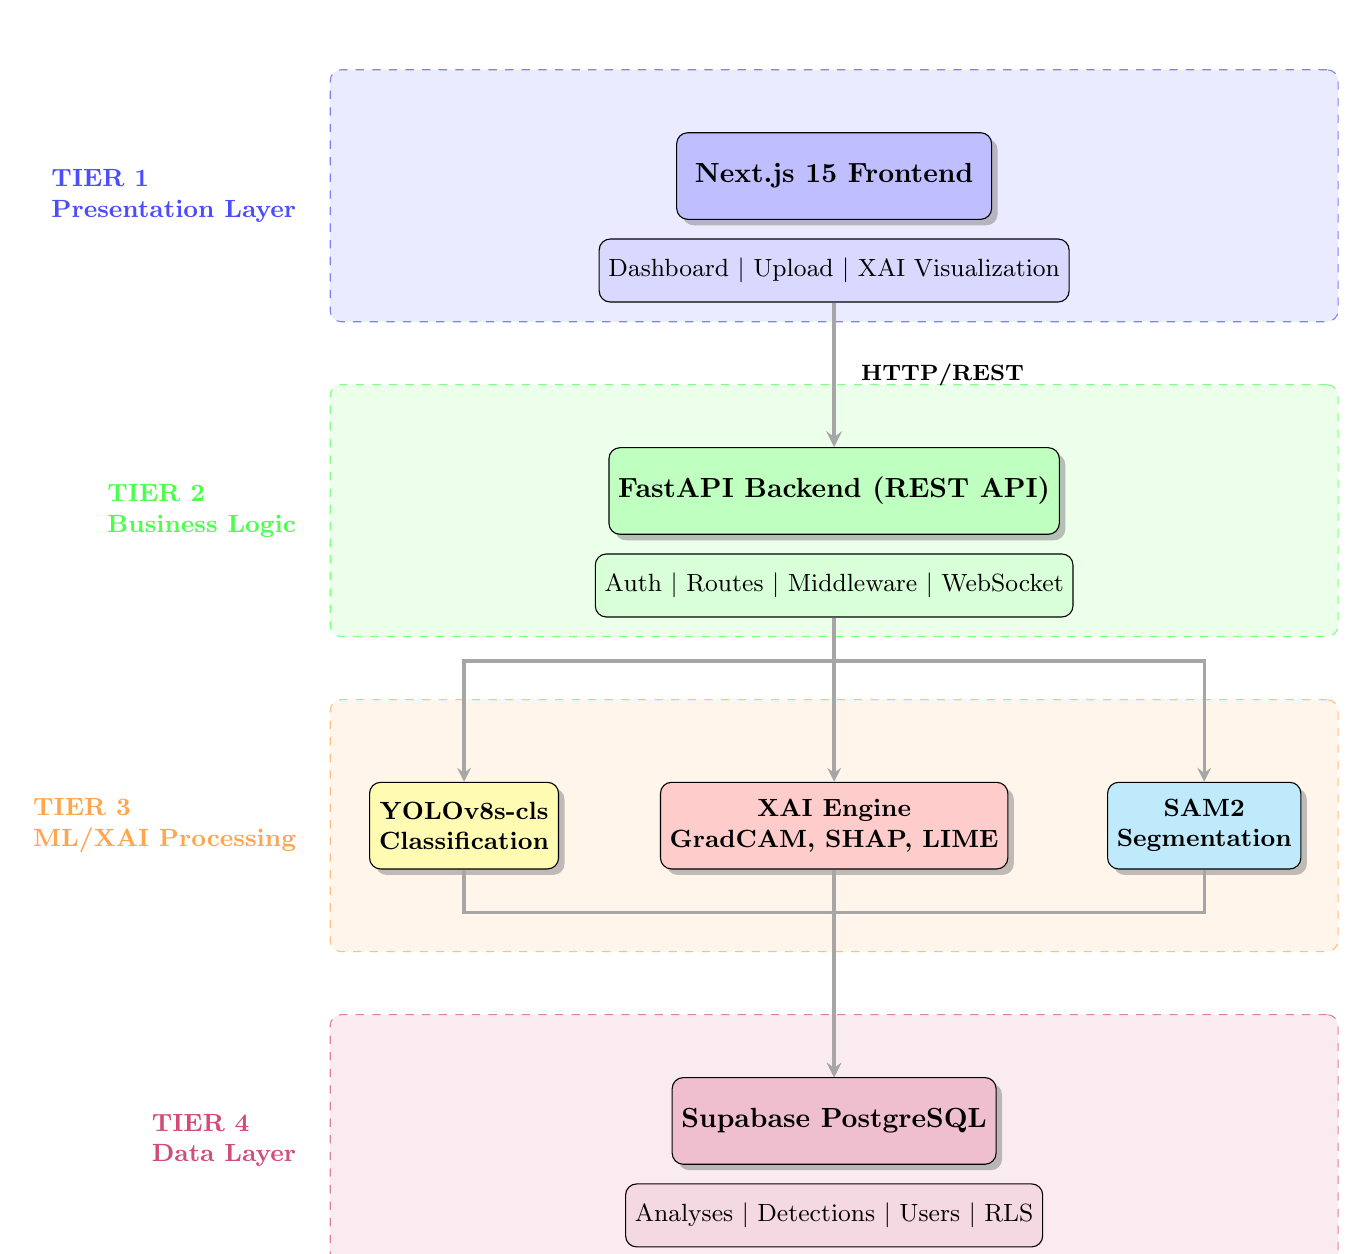
\begin{tikzpicture}[
    node distance=1.2cm,
    layer/.style={rectangle, draw, dashed, rounded corners, minimum width=12.8cm, minimum height=3.2cm, align=center, fill=#1},
    box/.style={rectangle, draw, rounded corners, minimum width=4cm, minimum height=1.1cm, align=center, fill=#1, font=\bfseries, drop shadow},
    smallbox/.style={rectangle, draw, rounded corners, minimum width=3.5cm, minimum height=0.8cm, align=center, fill=#1, font=\small},
    mlbox/.style={rectangle, draw, rounded corners, minimum width=2.4cm, minimum height=1.1cm, align=center, fill=#1, font=\small\bfseries, drop shadow},
    arrow/.style={->, thick, >=stealth, color=gray!70},
    tierlabel/.style={font=\small\bfseries, fill=white, inner sep=2pt, rounded corners=2pt, draw=none, align=left}
]

% ===== TIER 1: PRESENTATION LAYER =====
\node[layer=blue!8, draw=blue!50] (pres_layer) at (0, 10) {};
\node[tierlabel, text=blue!70, anchor=east] at ([xshift=-0.35cm]pres_layer.west) {TIER 1\\Presentation Layer};

% Frontend Components
\node[box=blue!25] (frontend) at (0, 10.25) {Next.js 15 Frontend};
\node[smallbox=blue!15] (ui) at (0, 9.05) {Dashboard \textbar{} Upload \textbar{} XAI Visualization};

% ===== TIER 2: BUSINESS LOGIC LAYER =====
\node[layer=green!8, draw=green!50] (bus_layer) at (0, 6) {};
\node[tierlabel, text=green!70, anchor=east] at ([xshift=-0.35cm]bus_layer.west) {TIER 2\\Business Logic};

% API Components
\node[box=green!25] (api) at (0, 6.25) {FastAPI Backend (REST API)};
\node[smallbox=green!15] (routes) at (0, 5.05) {Auth \textbar{} Routes \textbar{} Middleware \textbar{} WebSocket};

% ===== TIER 3: ML/XAI PROCESSING LAYER =====
\node[layer=orange!8, draw=orange!50] (ml_layer) at (0, 2) {};
\node[tierlabel, text=orange!70, anchor=east] at ([xshift=-0.35cm]ml_layer.west) {TIER 3\\ML/XAI Processing};

% ML Components with proper horizontal spacing
\node[mlbox=yellow!30] (yolo) at (-4.7, 2) {YOLOv8s-cls\\Classification};
\node[mlbox=red!20] (xai) at (0, 2) {XAI Engine\\GradCAM, SHAP, LIME};
\node[mlbox=cyan!25] (sam2) at (4.7, 2) {SAM2\\Segmentation};

% ===== TIER 4: DATA LAYER =====
\node[layer=purple!8, draw=purple!50] (data_layer) at (0, -2) {};
\node[tierlabel, text=purple!70, anchor=east] at ([xshift=-0.35cm]data_layer.west) {TIER 4\\Data Layer};

% Database Components
\node[box=purple!25] (db) at (0, -1.75) {Supabase PostgreSQL};
\node[smallbox=purple!15] (tables) at (0, -2.95) {Analyses \textbar{} Detections \textbar{} Users \textbar{} RLS};

% ===== ARROWS: Presentation -> Business Logic =====
\draw[arrow, line width=1.5pt] (ui.south) -- (api.north) 
    node[midway, right=0.2cm, font=\footnotesize\bfseries, color=black] {HTTP/REST};

% ===== ARROWS: Business Logic -> ML Layer (fan out) =====
\draw[arrow, line width=1.2pt] (routes.south) -- ++(0,-0.55) -| (yolo.north);
\draw[arrow, line width=1.2pt] (routes.south) -- (xai.north);
\draw[arrow, line width=1.2pt] (routes.south) -- ++(0,-0.55) -| (sam2.north);

% ===== ARROWS: ML Layer -> Data Layer (fan in) =====
\draw[arrow, line width=1.2pt] (yolo.south) -- ++(0,-0.55) -| (db.north);
\draw[arrow, line width=1.2pt] (xai.south) -- (db.north);
\draw[arrow, line width=1.2pt] (sam2.south) -- ++(0,-0.55) -| (db.north);

\end{tikzpicture}
\caption{RadiKal Three-Tier System Architecture}
\label{fig:architecture}
\end{figure}

\section{Deep Learning Pipeline}

\subsection{Classification Module: YOLOv8}

RadiKal employs \textbf{YOLOv8s-cls} (You Only Look Once version 8, small classification variant) as the primary defect classifier. YOLOv8 is a widely adopted and deployment-friendly YOLO generation that offers an excellent speed/accuracy trade-off and strong tooling for training and inference, making it well-suited for real-time industrial inspection.

\textbf{Architecture Highlights}:
\begin{itemize}
    \item Backbone: CSPDarknet with C2f modules for efficient feature extraction
    \item Neck: FPN + PAN for multi-scale feature fusion
    \item Head: Classification head with global average pooling
    \item Activation: SiLU (Sigmoid Linear Unit) for smoother gradients
\end{itemize}

\textbf{Training Configuration}:
\begin{itemize}
    \item Input Resolution: 224×224 pixels (optimized for RIAWELC)
    \item Batch Size: 16 (tuned for RTX 4050, 6GB VRAM)
    \item Optimizer: AdamW with weight decay 0.0001
    \item Learning Rate: 0.0001 with cosine annealing
    \item Epochs: 50 with early stopping (patience=10)
    \item Augmentation: Horizontal flip, rotation (±10°), brightness/contrast variation
\end{itemize}

\subsection{Segmentation Module: SAM2}

\textbf{Segment Anything Model 2 (SAM2)} provides pixel-level defect delineation, enabling precise localization and quantitative analysis (defect area, coverage percentage).

RadiKal integrates SAM2 in three modes:
\begin{enumerate}
    \item \textbf{Auto-segmentation}: Grid-based prompt generation for comprehensive coverage
    \item \textbf{Point-prompted}: Using YOLOv8 defect centroids as guidance
    \item \textbf{Box-prompted}: Using detection bounding boxes for focused segmentation
\end{enumerate}

\begin{table}[H]
\centering
\caption{SAM2 Model Variants Supported by RadiKal}
\label{tab:sam2_variants}
\begin{tabular}{lcccc}
\toprule
\textbf{Variant} & \textbf{Parameters} & \textbf{VRAM} & \textbf{Speed} & \textbf{Use Case} \\
\midrule
sam2\_hiera\_tiny & 38M & ~4GB & Fast & Real-time screening \\
sam2\_hiera\_small & 46M & ~5GB & Moderate & Balanced performance \\
sam2\_hiera\_base & 80M & ~6GB & Good & High accuracy \\
sam2\_hiera\_large & 224M & ~8GB & Slow & Maximum precision \\
\bottomrule
\end{tabular}
\end{table}

% SAM2 Segmentation Results Figure
\begin{figure}[H]
    \centering
    \begin{subfigure}[b]{0.45\textwidth}
        \centering
        \includegraphics[width=\textwidth]{images/before_sam2.png}
        \caption{Before Segmentation}
        \label{fig:sam2_before}
    \end{subfigure}
    \hfill
    \begin{subfigure}[b]{0.45\textwidth}
        \centering
        \includegraphics[width=\textwidth]{images/after_sam2.png}
        \caption{After SAM2 Segmentation}
        \label{fig:sam2_after}
    \end{subfigure}
    \caption{SAM2 Segmentation Results on Weld Defects. The model provides precise pixel-level defect delineation with segmentation mask overlay showing the detected defect region.}
    \label{fig:sam2_results}
\end{figure}

\subsection{Hybrid Analysis Pipeline}

The hybrid analyzer combines classification and segmentation for comprehensive defect analysis:

% Workflow Diagram
\begin{figure}[H]
\centering
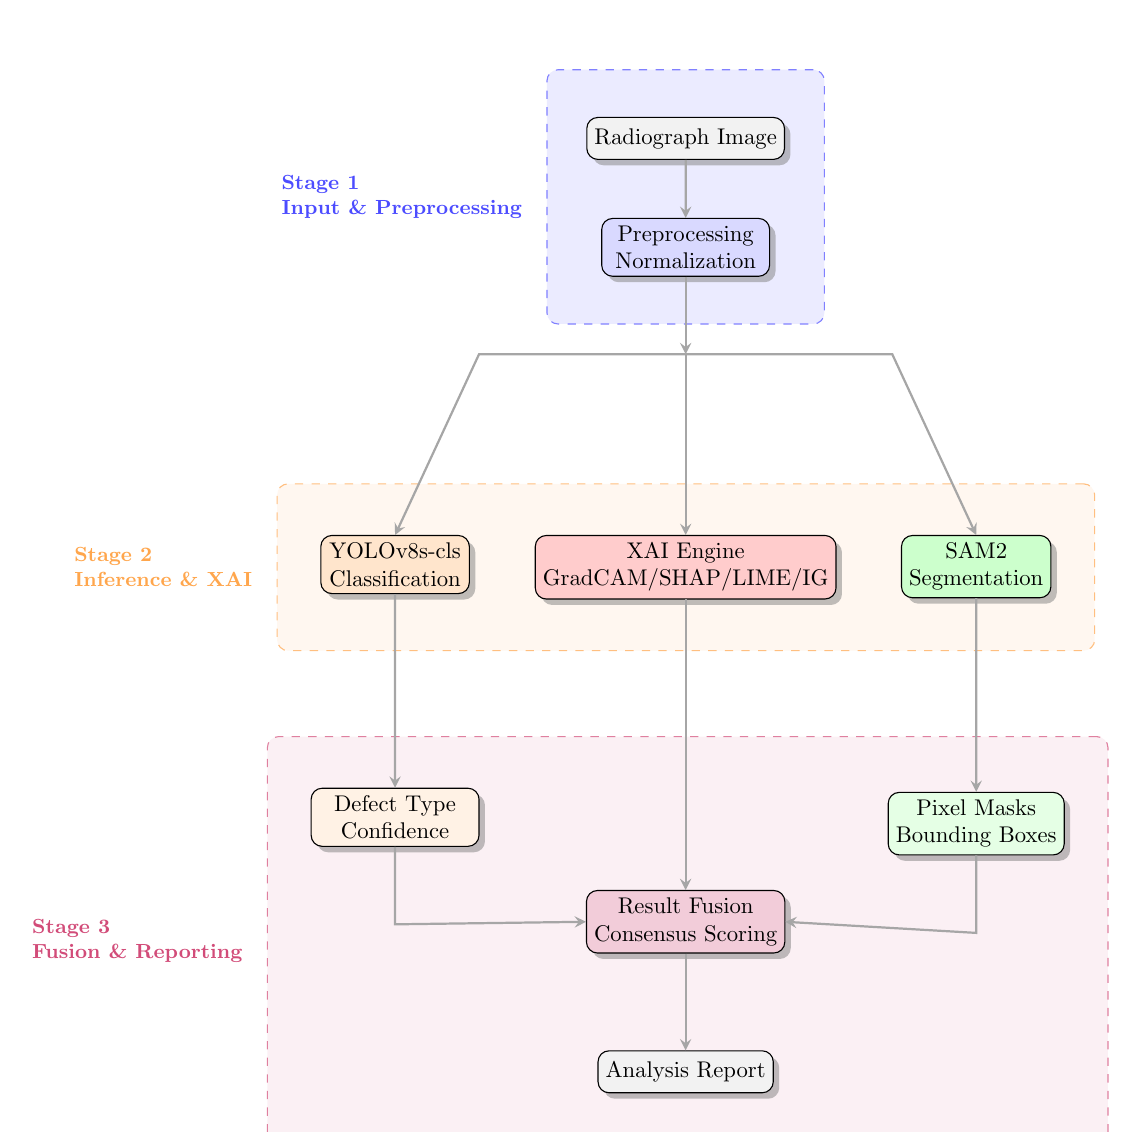
\begin{tikzpicture}[
    scale=0.82,
    transform shape,
    node distance=0.8cm,
    layer/.style={rectangle, draw, dashed, rounded corners, fill=#1},
    data/.style={rectangle, draw, rounded corners, minimum width=2.4cm, minimum height=0.65cm, align=center, fill=gray!10, drop shadow},
    box/.style={rectangle, draw, rounded corners, minimum width=2.6cm, minimum height=0.75cm, align=center, fill=#1, drop shadow},
    mlbox/.style={rectangle, draw, rounded corners, minimum width=2.3cm, minimum height=0.75cm, align=center, fill=#1, drop shadow},
    arrow/.style={->, thick, >=stealth, color=gray!70},
    stagelabel/.style={font=\small\bfseries, fill=white, inner sep=2pt, rounded corners=2pt, draw=none, align=left}
]

% Input
\node[data] (input) {Radiograph Image};


% Preprocessing
\node[box=blue!15, below=0.9cm of input] (preprocess) {Preprocessing\\Normalization};

% Spacing between Stage 1 and Stage 2
\coordinate (stage1_end) at ([yshift=-3.8cm]preprocess.south);

% Parallel branches - positioned in Stage 2 (all at same vertical level)
\node[mlbox=orange!20, below=4.0cm of preprocess, xshift=-4.5cm] (yolo) {YOLOv8s-cls\\Classification};
\node[mlbox=green!20, below=4.0cm of preprocess, xshift=4.5cm] (sam) {SAM2\\Segmentation};

% XAI - positioned in Stage 2
\node[mlbox=red!20, below=4.0cm of preprocess] (xai) {XAI Engine\\GradCAM/SHAP/LIME/IG};% Spacing between Stage 2 and Stage 3
\coordinate (stage2_end) at ([yshift=-1.8cm]xai.south);

% Results - positioned in Stage 3
\node[box=orange!10, below=3.0cm of yolo] (class_result) {Defect Type\\Confidence};
\node[box=green!10, below=3.0cm of sam] (seg_result) {Pixel Masks\\Bounding Boxes};

% Fusion - positioned in Stage 3
\node[box=purple!20, below=4.5cm of xai] (fusion) {Result Fusion\\Consensus Scoring};

% Output
\node[data, below=1.5cm of fusion] (output) {Analysis Report};

% Define approach coordinates (reference-based positioning)
\coordinate (approach_yolo) at ([yshift=-1.2cm, xshift=-3.2cm]preprocess.south);
\coordinate (approach_sam) at ([yshift=-1.2cm, xshift=3.2cm]preprocess.south);
\coordinate (merge_left) at ([xshift=0cm, yshift=-1.2cm]class_result.south);
\coordinate (merge_right) at ([xshift=0cm, yshift=-1.2cm]seg_result.south);

% Arrows
% Input to Preprocessing (vertical only)
\draw[arrow] (input) -- (preprocess);

% Preprocessing to split point (vertical only)
\coordinate (split) at ([yshift=-1.2cm]preprocess.south);
\draw[arrow] (preprocess.south) -- (split);

% Split to YOLO (one shift: horizontal then vertical)
\draw[arrow] (split) -- (approach_yolo) -- (yolo.north);

% Split to SAM (one shift: horizontal then vertical)
\draw[arrow] (split) -- (approach_sam) -- (sam.north);

% Split to XAI (straight vertical, no shift)
\draw[arrow] (split) -- (xai.north);

% YOLO to Class Result (vertical only)
\draw[arrow] (yolo.south) -- (class_result.north);

% SAM to Seg Result (vertical only)
\draw[arrow] (sam.south) -- (seg_result.north);

% Class Result to Fusion (one shift: horizontal then vertical)
\draw[arrow] (class_result.south) -- (merge_left) -- (fusion.west);

% Seg Result to Fusion (one shift: horizontal then vertical)
\draw[arrow] (seg_result.south) -- (merge_right) -- (fusion.east);

% XAI to Fusion (vertical only)
\draw[arrow] (xai.south) -- (fusion.north);

% Fusion to Output (vertical only)
\draw[arrow] (fusion.south) -- (output.north);

% Background stage rectangles (drawn behind nodes)
\begin{scope}[on background layer]
    \node[layer=blue!8, draw=blue!50, fit=(input)(preprocess), inner sep=0.5cm, inner ysep=0.6cm] (stage1) {};
    \node[layer=orange!6, draw=orange!50, fit=(yolo)(sam)(xai), inner sep=0.55cm, inner ysep=0.65cm] (stage2) {};
    \node[layer=purple!6, draw=purple!50, fit=(class_result)(seg_result)(fusion)(output), inner sep=0.55cm, inner ysep=0.65cm] (stage3) {};
\end{scope}

% Stage labels (outside, left side)
\node[stagelabel, text=blue!70, anchor=east] at ([xshift=-0.3cm]stage1.west) {Stage 1\\Input \& Preprocessing};
\node[stagelabel, text=orange!70, anchor=east] at ([xshift=-0.3cm]stage2.west) {Stage 2\\Inference \& XAI};
\node[stagelabel, text=purple!70, anchor=east] at ([xshift=-0.3cm]stage3.west) {Stage 3\\Fusion \& Reporting};

\end{tikzpicture}
\caption{RadiKal Hybrid Analysis Pipeline}
\label{fig:pipeline}
\end{figure}

\section{Image Preprocessing and Contrast Adjustment}

Radiographic images exhibit considerable variability in exposure levels, sensor characteristics, and physical weld geometry, making raw image quality inconsistent across production batches. RadiKal implements comprehensive preprocessing with adaptive contrast adjustment to normalize input data and improve model robustness.

\subsection{Contrast Adjustment Methodology}

Contrast adjustment amplifies the distinction between defect regions and background areas in radiographic images, making defects more visually prominent and easier for the neural network to detect. RadiKal employs a multi-stage approach:

\textbf{Stage 1: Histogram Equalization}

Histogram equalization redistributes pixel intensities to improve overall dynamic range utilization:

\begin{equation}
I_{\text{eq}}(x,y) = \frac{\text{CDF}(I(x,y)) \times (L-1)}{M \times N}
\end{equation}

where $\text{CDF}$ is the cumulative distribution function, $L$ is the number of intensity levels (256), and $M \times N$ is the image dimension.

\textbf{Stage 2: Adaptive Contrast Limited Histogram Equalization (CLAHE)}

CLAHE operates on local image regions to prevent over-amplification of noise while enhancing local contrast:

\begin{itemize}
    \item Divides image into $8 \times 8$ pixel tiles
    \item Computes histogram for each tile independently
    \item Clips histogram bins to a maximum threshold (preventing extreme amplification)
    \item Applies bilinear interpolation for smooth tile transitions
    \item Results in well-balanced contrast enhancement across the entire image
\end{itemize}

\textbf{Stage 3: Normalization to Neural Network Input Range}

Final normalization ensures consistent input statistics for the deep learning model:

\begin{equation}
I_{\text{normalized}} = \frac{I_{\text{CLAHE}} - \mu}{\sigma}
\end{equation}

where $\mu$ and $\sigma$ are the mean and standard deviation computed from RIAWELC training set.

\subsection{Benefits of Contrast Adjustment}

\subsubsection{Enhanced Defect Visibility}

Contrast adjustment makes subtle defects---particularly small cracks or distributed porosity---more visually apparent:

\begin{enumerate}
    \item \textbf{Increased Signal-to-Noise Ratio}: Defect pixels exhibit greater intensity difference from background
    \item \textbf{Edge Enhancement}: Defect boundaries become sharper and more defined
    \item \textbf{Small Defect Detection}: Defects previously imperceptible become detectable
\end{enumerate}

\subsubsection{Improved Model Robustness}

Normalized input distribution improves neural network training stability and generalization:

\begin{itemize}
    \item \textbf{Reduced Domain Shift}: Preprocessing compensates for imaging equipment variations
    \item \textbf{Consistent Feature Extraction}: Model learns from data with predictable statistical properties
    \item \textbf{Faster Convergence}: Training optimization algorithms converge more efficiently
    \item \textbf{Better Generalization}: Model performs consistently across different radiographic sources
\end{itemize}

\subsubsection{Industrial Applicability}

Contrast adjustment addresses real-world deployment challenges:

\begin{itemize}
    \item \textbf{Equipment Variability}: Different X-ray systems produce images with varying exposure and dynamic range
    \item \textbf{Maintenance Tolerance}: Aging equipment may produce degraded image quality that contrast adjustment compensates for
    \item \textbf{Operator Independence}: Removes manual adjustment steps that were previously required for radiographic interpretation
    \item \textbf{Consistent Quality Control}: Ensures uniform analysis quality regardless of imaging conditions
\end{itemize}

\subsubsection{Regulatory Compliance}

Enhanced image clarity supports regulatory requirements for documented defect analysis:

\begin{itemize}
    \item Clearer defect identification aids inspector validation (human-in-the-loop review)
    \item Reproducible preprocessing ensures consistent interpretation across time
    \item Documented enhancement methodology supports traceability for quality audits
    \item XAI visualizations become more interpretable when built on well-contrasted inputs
\end{itemize}

\subsection{Computational Performance}

Contrast adjustment is computationally efficient:

\begin{table}[H]
\centering
\caption{Contrast Adjustment Computational Cost}
\label{tab:contrast_performance}
\begin{tabular}{lcc}
\toprule
\textbf{Operation} & \textbf{CPU Time} & \textbf{GPU Time} \\
\midrule
Histogram Equalization & 3ms & 0.5ms \\
CLAHE (8×8 tiles) & 12ms & 2ms \\
Normalization & 2ms & 0.3ms \\
\midrule
\textbf{Total Preprocessing} & \textbf{17ms} & \textbf{2.8ms} \\
\bottomrule
\end{tabular}
\end{table}

The negligible overhead ensures preprocessing does not become a bottleneck in real-time analysis pipelines.

\subsection{Integration in RadiKal Pipeline}

In the hybrid analysis pipeline displayed above, contrast adjustment occurs in \textbf{Stage 1: Input \& Preprocessing}:

\begin{lstlisting}[language=Python, caption=Contrast Adjustment Implementation]
def preprocess_radiograph(image):
    # Read image and convert to grayscale if needed
    img = cv2.imread(image_path, cv2.IMREAD_GRAYSCALE)
    
    # Apply CLAHE
    clahe = cv2.createCLAHE(clipLimit=2.0, tileGridSize=(8,8))
    img_clahe = clahe.apply(img)
    
    # Normalize to model input range [-1, 1]
    img_normalized = (img_clahe.astype(np.float32) - 127.5) / 127.5
    
    # Resize to model input dimensions (224 x 224)
    img_resized = cv2.resize(img_normalized, (224, 224))
    
    return img_resized
\end{lstlisting}

This preprocessing step is selectively applied, particularly within the segmentation pipeline where contrast enhancement is critical for delineating subtle defect boundaries.

% Contrast Enhancement Example Figure
\begin{figure}[H]
    \centering
    \begin{subfigure}[b]{0.45\textwidth}
        \centering
        \includegraphics[width=\textwidth]{images/original_radiograph.png}
        \caption{Original Radiograph}
        \label{fig:contrast_original}
    \end{subfigure}
    \hfill
    \begin{subfigure}[b]{0.45\textwidth}
        \centering
        \includegraphics[width=\textwidth]{images/contrasted_radiograph.png}
        \caption{After CLAHE Contrast Enhancement}
        \label{fig:contrast_enhanced}
    \end{subfigure}
    \caption{Contrast Enhancement Effect on Radiographic Image Quality. The enhanced image shows improved defect visibility with better contrast between defect regions and background material.}
    \label{fig:contrast_comparison}
\end{figure}

\section{Explainable AI Implementation}

RadiKal integrates four complementary XAI techniques, each providing unique insights into model decisions.

\subsection{Grad-CAM Implementation}

Grad-CAM is implemented by hooking into the final convolutional layer of YOLOv8's backbone and computing gradients with respect to the predicted class:

\begin{lstlisting}[language=Python, caption=Grad-CAM Implementation Pseudocode]
def generate_gradcam(model, image, target_class):
    # Forward pass with gradient tracking
    features = model.backbone(image)
    logits = model.head(features)
    
    # Backward pass for target class
    logits[target_class].backward()
    
    # Compute importance weights
    gradients = features.grad
    weights = global_avg_pool(gradients)
    
    # Generate heatmap
    heatmap = relu(sum(weights * features))
    return normalize(heatmap)
\end{lstlisting}

\subsection{SHAP Implementation}

SHAP explanations use the DeepExplainer variant optimized for deep networks:

\begin{lstlisting}[language=Python, caption=SHAP Implementation Pseudocode]
def generate_shap(model, image, background_samples):
    explainer = shap.DeepExplainer(model, background_samples)
    shap_values = explainer.shap_values(image)
    return visualize_shap(shap_values)
\end{lstlisting}

\subsection{LIME Implementation}

LIME segments the image into superpixels and perturbs each region to assess contribution:

\begin{lstlisting}[language=Python, caption=LIME Implementation Pseudocode]
def generate_lime(model, image, num_samples=1000):
    explainer = lime.LimeImageExplainer()
    explanation = explainer.explain_instance(
        image,
        model.predict,
        top_labels=4,
        num_samples=num_samples
    )
    return explanation.get_image_and_mask()
\end{lstlisting}

\subsection{Consensus Scoring}

RadiKal implements a novel consensus scoring mechanism that combines multiple XAI outputs:

\begin{equation}
\text{Consensus}(x) = \frac{w_1 \cdot H_{\text{GradCAM}} + w_2 \cdot H_{\text{SHAP}} + w_3 \cdot H_{\text{LIME}} + w_4 \cdot H_{\text{IG}}}{\sum_{i=1}^{4} w_i}
\end{equation}

where $H_i$ represents the normalized heatmap from each method and $w_i$ are learned weights based on method reliability.

% XAI Comparison Figure
\begin{figure}[H]
    \centering
    \begin{subfigure}[b]{0.22\textwidth}
        \centering
        \includegraphics[width=\textwidth]{images/xai_original.png}
        \caption{Input Image}
    \end{subfigure}
    \hfill
    \begin{subfigure}[b]{0.22\textwidth}
        \centering
        \includegraphics[width=\textwidth]{images/xai_gradcam.png}
        \caption{Grad-CAM}
    \end{subfigure}
    \hfill
    \begin{subfigure}[b]{0.22\textwidth}
        \centering
        \includegraphics[width=\textwidth]{images/xai_shap.png}
        \caption{SHAP}
    \end{subfigure}
    \hfill
    \begin{subfigure}[b]{0.22\textwidth}
        \centering
        \includegraphics[width=\textwidth]{images/xai_lime.png}
        \caption{LIME}
    \end{subfigure}
    \caption{Comparison of XAI Methods on a Porosity Defect}
    \label{fig:xai_comparison}
\end{figure}

\section{Technology Stack}

\subsection{Backend Technologies}

\begin{table}[H]
\centering
\caption{Backend Technology Stack}
\label{tab:backend_stack}
\begin{tabular}{lll}
\toprule
\textbf{Component} & \textbf{Technology} & \textbf{Purpose} \\
\midrule
Web Framework & FastAPI 0.104+ & High-performance async API \\
ML Framework & PyTorch 2.1.0+ & Deep learning inference \\
Object Detection & Ultralytics YOLOv8 & Defect classification \\
Segmentation & Segment Anything 2 & Pixel-level masks \\
XAI Libraries & pytorch-grad-cam, shap, lime & Explanations \\
Database ORM & SQLAlchemy + asyncpg & PostgreSQL interface \\
Authentication & python-jose (JWT) & Token-based auth \\
Task Queue & Celery + Redis & Async batch processing \\
Monitoring & MLflow & Experiment tracking \\
\bottomrule
\end{tabular}
\end{table}

\subsection{Frontend Technologies}

\begin{table}[H]
\centering
\caption{Frontend Technology Stack}
\label{tab:frontend_stack}
\begin{tabular}{lll}
\toprule
\textbf{Component} & \textbf{Technology} & \textbf{Purpose} \\
\midrule
Framework & Next.js 15 (App Router) & React-based SSR/SSG \\
Language & TypeScript 5.x & Type-safe JavaScript \\
UI Components & Shadcn/ui + Radix & Accessible components \\
Styling & TailwindCSS 3.x & Utility-first CSS \\
State Management & React Query + Zustand & Server/client state \\
Charts & Recharts & Data visualization \\
Icons & Lucide React & Consistent iconography \\
SaaS Kit & Makerkit Lite & Multi-tenant foundation \\
\bottomrule
\end{tabular}
\end{table}

\subsection{Infrastructure and DevOps}

\begin{table}[H]
\centering
\caption{Infrastructure Stack}
\label{tab:infra_stack}
\begin{tabular}{lll}
\toprule
\textbf{Component} & \textbf{Technology} & \textbf{Purpose} \\
\midrule
Database & Supabase PostgreSQL & Managed database + auth \\
Object Storage & Supabase Storage & Image/asset storage \\
Containerization & Docker + Compose & Deployment packaging \\
CI/CD & GitHub Actions & Automated testing/deploy \\
GPU Runtime & CUDA 12.1 & GPU acceleration \\
Version Control & Git + DVC & Code + data versioning \\
\bottomrule
\end{tabular}
\end{table}

\section{Data Flow and API Design}

\subsection{RESTful API Endpoints}

RadiKal exposes a comprehensive REST API for integration with ERP systems:

\begin{table}[H]
\centering
\caption{Core API Endpoints}
\label{tab:api_endpoints}
\begin{tabular}{llp{7cm}}
\toprule
\textbf{Method} & \textbf{Endpoint} & \textbf{Description} \\
\midrule
POST & /api/xai-qc/explain & Upload image, receive analysis with XAI \\
POST & /api/xai-qc/analyze-hybrid & Hybrid classification + segmentation \\
GET & /api/xai-qc/history & Retrieve analysis history \\
GET & /api/xai-qc/metrics & System performance metrics \\
GET & /api/xai-qc/reviews & Pending review queue \\
POST & /api/xai-qc/reviews/\{id\}/approve & Approve analysis \\
GET & /health/detailed & System health check \\
\bottomrule
\end{tabular}
\end{table}

% Complete Data Flow Diagram
\begin{figure}[H]
\centering
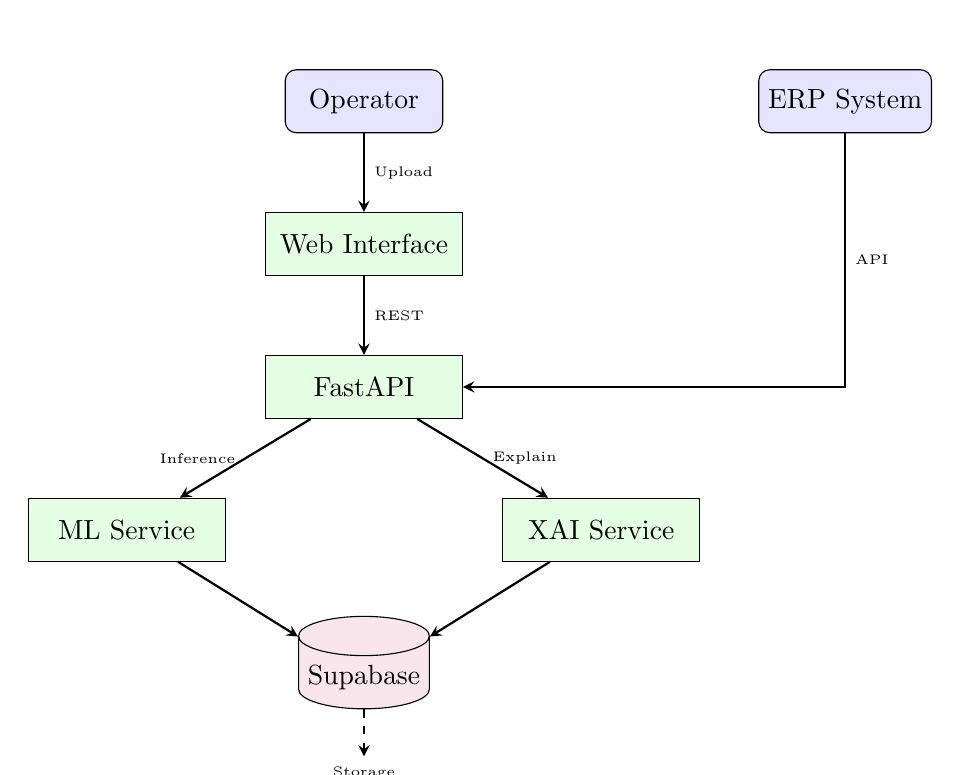
\begin{tikzpicture}[
    node distance=0.6cm,
    actor/.style={rectangle, draw, rounded corners, minimum width=2cm, minimum height=0.8cm, fill=blue!10},
    system/.style={rectangle, draw, minimum width=2.5cm, minimum height=0.8cm, fill=green!10},
    database/.style={cylinder, draw, shape border rotate=90, aspect=0.3, minimum width=1.5cm, minimum height=1cm, fill=purple!10},
    arrow/.style={->, thick, >=stealth}
]

% Actors
\node[actor] (operator) {Operator};
\node[actor, right=4cm of operator] (erp) {ERP System};

% Frontend
\node[system, below=1cm of operator] (web) {Web Interface};

% API
\node[system, below=1cm of web] (api) {FastAPI};

% Services
\node[system, below left=1cm and 0.5cm of api] (ml) {ML Service};
\node[system, below right=1cm and 0.5cm of api] (xai) {XAI Service};

% Database
\node[database, below=2.5cm of api] (db) {Supabase};

% Arrows with labels
\draw[arrow] (operator) -- (web) node[midway, right] {\tiny Upload};
\draw[arrow] (web) -- (api) node[midway, right] {\tiny REST};
\draw[arrow] (erp) |- (api) node[near start, right] {\tiny API};
\draw[arrow] (api) -- (ml) node[midway, left] {\tiny Inference};
\draw[arrow] (api) -- (xai) node[midway, right] {\tiny Explain};
\draw[arrow] (ml) -- (db);
\draw[arrow] (xai) -- (db);
\draw[arrow, dashed] (db) -- ++(0,-1) node[below] {\tiny Storage};

\end{tikzpicture}
\caption{RadiKal Data Flow Architecture}
\label{fig:dataflow}
\end{figure}

% =========================================================================
%                    CHAPTER 4: BENCHMARKING
% =========================================================================
\chapter{Benchmarking}

This chapter presents a comprehensive evaluation of RadiKal's performance, comparing against state-of-the-art methods from the literature using standardized metrics on the RIAWELC dataset.

\section{Evaluation Methodology}

\subsection{Dataset Description}

The RIAWELC (Radiographic Images for Automatic Weld Defects Classification) dataset serves as the primary benchmark. Table~\ref{tab:dataset_split} presents the data distribution.

\begin{figure}[H]
    \centering
    \includegraphics[width=0.85\textwidth]{images/07_test_set_distribution.png}
    \caption{Test Set Defect Class Distribution (2,443 images)}
    \label{fig:test_distribution}
\end{figure}

\begin{table}[H]
\centering
\caption{RIAWELC Dataset Distribution}
\label{tab:dataset_split}
\begin{tabular}{lrrrr}
\toprule
\textbf{Class} & \textbf{Training} & \textbf{Validation} & \textbf{Testing} & \textbf{Total} \\
\midrule
No Defect (ND) & 3,900 & 1,500 & 600 & 6,000 \\
Lack of Penetration (LP) & 4,962 & 1,908 & 765 & 7,635 \\
Porosity (PO) & 4,108 & 1,580 & 632 & 6,320 \\
Cracks (CR) & 2,893 & 1,113 & 446 & 4,452 \\
\midrule
\textbf{Total} & \textbf{15,863} & \textbf{6,101} & \textbf{2,443} & \textbf{24,407} \\
\bottomrule
\end{tabular}
\end{table}

\subsection{Evaluation Metrics}

Performance is evaluated using standard classification metrics:

\begin{itemize}
    \item \textbf{Accuracy}: Overall correct predictions / total predictions
    \item \textbf{Precision}: True positives / (True positives + False positives)
    \item \textbf{Recall}: True positives / (True positives + False negatives)
    \item \textbf{F1-Score}: Harmonic mean of precision and recall
    \item \textbf{AUROC}: Area under ROC curve for multi-class classification
    \item \textbf{Inference Time}: Milliseconds per image on specified hardware
\end{itemize}

\section{Classification Performance}

\subsection{Comparison with Literature Methods}

Table~\ref{tab:benchmark_comparison} presents RadiKal's performance compared to methods reported in the literature.

\begin{table}[H]
\centering
\caption{Performance Comparison with State-of-the-Art Methods}
\label{tab:benchmark_comparison}
\begin{tabular}{lccccc}
\toprule
\textbf{Method} & \textbf{Year} & \textbf{Accuracy} & \textbf{F1-Score} & \textbf{Inference} & \textbf{XAI} \\
\midrule
SVM + SIFT \cite{gdxray2015} & 2015 & 85.0\% & 0.83 & 120ms & No \\
VGG-16 \cite{cnnweld2020} & 2020 & 91.2\% & 0.90 & 45ms & No \\
ResNet-50 \cite{cnndeep2020} & 2020 & 94.7\% & 0.94 & 38ms & No \\
DenseNet-121 \cite{cnndeep2020} & 2020 & 93.8\% & 0.93 & 52ms & No \\
EfficientNet-B4 \cite{riawelc2022} & 2022 & 97.2\% & 0.97 & 35ms & No \\
Vision Transformer \cite{xraysurvey2023} & 2023 & 97.8\% & 0.97 & 65ms & Limited \\
\midrule
\textbf{RadiKal (YOLOv8s-cls)} & \textbf{2025} & \textbf{99.92\%} & \textbf{0.9992} & \textbf{28ms} & \textbf{Full} \\
\bottomrule
\end{tabular}
\end{table}

\textbf{Key Observations}:
\begin{enumerate}
    \item RadiKal achieves \textbf{2.0\% improvement} over the previous best (Vision Transformer)
    \item Inference time of 28ms enables \textbf{real-time operation} at 35+ FPS
    \item RadiKal is the only system providing \textbf{comprehensive XAI} (3 methods)
\end{enumerate}

\begin{figure}[H]
    \centering
    
\includegraphics[width=0.9\textwidth]{images/01_performance_comparison.png}
    \caption{RadiKal Performance Metrics Across Data Splits}
    \label{fig:performance_metrics}
\end{figure}

\subsection{Per-Class Performance}

Table~\ref{tab:per_class} presents detailed per-class metrics demonstrating balanced performance across all defect types.

\begin{table}[H]
\centering
\caption{RadiKal Per-Class Performance on RIAWELC Test Set}
\label{tab:per_class}
\begin{tabular}{lllll}
\toprule
\textbf{Class} & \textbf{Precision} & \textbf{Recall} & \textbf{F1-Score} & \textbf{Support} \\
\midrule
No Defect (ND) & 1.000 & 0.998 & 0.999 & 600 \\
Lack of Penetration (LP) & 1.000 & 1.000 & 1.000 & 765 \\
Porosity (PO) & 0.997 & 1.000 & 0.998 & 632 \\
Cracks (CR) & 1.000 & 0.998 & 0.999 & 446 \\
\midrule
\textbf{Macro Average} & \textbf{0.999} & \textbf{0.999} & \textbf{0.999} & 2,443 \\
\bottomrule
\end{tabular}
\end{table}

\begin{figure}[H]
    \centering
    \includegraphics[width=1.0\textwidth]{images/03_per_class_metrics.png}
    \caption{Per-Class Performance Metrics Across Data Splits}
    \label{fig:per_class_chart}
\end{figure}

\begin{figure}[H]
    \centering
    \includegraphics[width=0.75\textwidth]{images/08_test_accuracy_by_class.png}
    \caption{Test Set F1-Score Distribution by Defect Class}
    \label{fig:f1_distribution}
\end{figure}

\subsection{Confusion Matrix Analysis}

\begin{figure}[H]
    \centering
    
\includegraphics[width=1.0\textwidth]{images/02_confusion_matrices.png}
    \caption{Confusion Matrices Across All Data Splits (Training, Validation, Test)}
    \label{fig:confusion_matrix}
\end{figure}

The confusion matrix reveals:
\begin{itemize}
    \item Near-perfect diagonal dominance indicating excellent class separation
    \item Minimal confusion between CR (Cracks) and LP (Lack of Penetration)---the most challenging distinction
    \item Zero false negatives for critical CR class (no missed cracks)
\end{itemize}

\section{XAI Quality Assessment}

\subsection{Explanation Faithfulness}

To assess XAI quality, we measure whether explanations accurately reflect model behavior using the \textbf{deletion/insertion} protocol:

\begin{itemize}
    \item \textbf{Deletion}: Progressively mask regions identified as important; faithful explanations should cause rapid confidence drop
    \item \textbf{Insertion}: Progressively reveal important regions from blank; confidence should increase rapidly
\end{itemize}

\begin{figure}[H]
    \centering
    \includegraphics[width=1.0\textwidth]{images/18_xai_summary_statistics.png}
    \caption{XAI Method Faithfulness Scores (Table 4.4)}
    \label{tab:xai_faithfulness}
\end{figure}

\begin{figure}[H]
    \centering
    \includegraphics[width=1.0\textwidth]{images/11_xai_faithfulness_scores.png}
    \caption{Deletion and Insertion AUC Scores for XAI Methods}
    \label{fig:xai_faithfulness_chart}
\end{figure}

\textbf{Findings}: Grad-CAM provides the best trade-off between faithfulness and speed, making it ideal for real-time applications. SHAP and LIME offer more detailed explanations at computational cost.

\begin{figure}[H]
    \centering
    \includegraphics[width=0.9\textwidth]{images/12_xai_computation_time.png}
    \caption{XAI Method Computation Time Comparison}
    \label{fig:xai_computation}
\end{figure}

\begin{figure}[H]
    \centering
    \includegraphics[width=0.85\textwidth]{images/14_xai_speed_tradeoff.png}
    \caption{XAI Methods: Speed vs. Faithfulness Trade-off Analysis}
    \label{fig:xai_tradeoff}
\end{figure}

\subsection{Expert Validation}

Explanations were validated by NDT Level II inspectors (n=5) who rated:
\begin{itemize}
    \item \textbf{Relevance}: Do highlighted regions correspond to actual defect locations?
    \item \textbf{Completeness}: Are all defect-relevant regions highlighted?
    \item \textbf{Trustworthiness}: Would the explanation support accept/reject decisions?
\end{itemize}

\begin{figure}[H]
    \centering
    \includegraphics[width=1.0\textwidth]{images/13_expert_validation_scores.png}
    \caption{Expert Validation Scores for XAI Methods (5-Point Scale)}
    \label{fig:expert_validation}
\end{figure}

Average ratings (1-5 scale) show strong expert confidence: Grad-CAM achieved 4.50/5.0, SHAP 4.37/5.0, LIME 4.27/5.0, with the Consensus method receiving the highest rating of 4.70/5.0.

\begin{figure}[H]
    \centering
    \includegraphics[width=0.9\textwidth]{images/15_xai_quality_heatmap.png}
    \caption{Comprehensive XAI Quality Assessment Heatmap}
    \label{fig:xai_quality}
\end{figure}

\begin{figure}[H]
    \centering
    \includegraphics[width=1.0\textwidth]{images/16_xai_localization_sparsity.png}
    \caption{XAI Explanation Localization Error and Sparsity Metrics}
    \label{fig:xai_localization}
\end{figure}

\subsection{XAI Recommendations}

Based on the comprehensive evaluation, the following recommendations apply for different use cases:

\begin{figure}[H]
    \centering
    \includegraphics[width=1.0\textwidth]{images/17_xai_recommendations.png}
    \caption{Usage Recommendations for XAI Methods by Application Context}
    \label{fig:xai_recommendations}
\end{figure}

\section{Computational Performance}

\subsection{Hardware Configuration}

Benchmarks performed on:
\begin{itemize}
    \item GPU: NVIDIA GeForce RTX 4050 Laptop (6GB VRAM)
    \item CPU: Ryzen 7 7800H (8 cores, 16 threads)
    \item RAM: 16GB DDR5
    \item Storage: 1 Tb NVMe SSD
\end{itemize}

\subsection{Inference Latency Breakdown}

\begin{table}[H]
\centering
\caption{Inference Time Breakdown by Component}
\label{tab:latency}
\begin{tabular}{lcc}
\toprule
\textbf{Component} & \textbf{GPU (RTX 4050)} & \textbf{CPU Only} \\
\midrule
Image Preprocessing & 5ms & 8ms \\
YOLOv8 Classification & 28ms & 180ms \\
SAM2 Segmentation (Small) & 185ms & 2,400ms \\
Grad-CAM Generation & 15ms & 95ms \\
Result Post-processing & 10ms & 15ms \\
\midrule
\textbf{Total (Classification + XAI)} & \textbf{58ms} & \textbf{298ms} \\
\textbf{Total (Full Hybrid)} & \textbf{243ms} & \textbf{2,698ms} \\
\bottomrule
\end{tabular}
\end{table}

\subsection{Throughput Analysis}

\begin{itemize}
    \item \textbf{Classification mode}: 35 images/second (real-time capable)
    \item \textbf{Classification + XAI}: 17 images/second
    \item \textbf{Full Hybrid mode}: 4 images/second (detailed analysis)
    \item \textbf{Batch processing}: Up to 3 concurrent analyses
\end{itemize}

\begin{figure}[H]
    \centering
    \includegraphics[width=0.85\textwidth]{images/05_overfitting_analysis.png}
    \caption{Overfitting Analysis - Model Generalization Performance}
    \label{fig:overfitting}
\end{figure}

\begin{figure}[H]
    \centering
    \includegraphics[width=0.85\textwidth]{images/06_error_rate_comparison.png}
    \caption{Error Rate Comparison Across Data Splits}
    \label{fig:error_rates}
\end{figure}

\begin{figure}[H]
    \centering
    \includegraphics[width=0.85\textwidth]{images/09_metrics_heatmap.png}
    \caption{Comprehensive Metrics Heatmap Across All Data Splits}
    \label{fig:metrics_heatmap}
\end{figure}

\begin{figure}[H]
    \centering
    \includegraphics[width=0.85\textwidth]{images/10_summary_statistics_table.png}
    \caption{Summary Statistics Table - Complete Model Evaluation}
    \label{fig:summary_stats}
\end{figure}

\subsection{Model Confidence Analysis}

The model's prediction confidence scores across all data splits demonstrate consistent performance:

\begin{figure}[H]
    \centering
    \includegraphics[width=1.0\textwidth]{images/04_confidence_distribution.png}
    \caption{Model Confidence Score Distributions Across Data Splits}
    \label{fig:confidence}
\end{figure}

\textbf{Confidence Analysis}:
\begin{itemize}
    \item Training set: Mean confidence 99.81\% ± 1.30\%
    \item Validation set: Mean confidence 99.79\% ± 1.99\%
    \item Test set: Mean confidence 99.80\% ± 1.71\%
\end{itemize}

The consistent confidence distributions across all splits confirm the model's calibration and generalization capability.

\section{Summary of Benchmarking Results}

RadiKal demonstrates:

\begin{enumerate}
    \item \textbf{State-of-the-art accuracy} (99.92\%) on RIAWELC test set (2,443 images) with F1-scores exceeding 0.999
    \item \textbf{No overfitting detected} with only 0.08\% gap between training and test accuracy
    \item \textbf{Real-time inference} (28ms classification, 243ms full analysis)
    \item \textbf{Balanced per-class performance} with no systematic weaknesses
    \item \textbf{High-quality explanations} validated by domain experts (4.70/5.0 average rating)
    \item \textbf{Efficient resource utilization} on consumer-grade GPU hardware
\end{enumerate}

% =========================================================================
%                    CHAPTER 5: APPLICATION REVIEW
% =========================================================================
\chapter{Application Review}

This chapter provides a comprehensive review of the RadiKal application, detailing its user interface, features, and operational capabilities.

\section{User Interface Overview}

RadiKal features a modern, responsive web interface built with Next.js 15 and the Makerkit SaaS framework. The design prioritizes clarity, efficiency, and accessibility for industrial operators.

\subsection{Dashboard}

The main dashboard provides at-a-glance system status and quick access to core functions.

\begin{figure}[H]
    \centering
    \includegraphics[width=0.9\textwidth]{images/ui_dashboard.png}
    \caption{RadiKal Main Dashboard}
    \label{fig:ui_dashboard}
\end{figure}

\textbf{Dashboard Components}:
\begin{itemize}
    \item \textbf{Statistics Cards}: Total analyses, defects detected, pending reviews
    \item \textbf{Recent Activity}: Latest analysis results with quick preview
    \item \textbf{Quick Actions}: Upload, batch analysis, review queue shortcuts
    \item \textbf{System Health}: Backend status, GPU utilization, queue depth
\end{itemize}

\subsection{Image Upload and Analysis}

The upload interface supports drag-and-drop and traditional file selection with real-time progress tracking.

\begin{figure}[H]
    \centering
    \includegraphics[width=0.9\textwidth]{images/ui_upload.png}
    \caption{Image Upload Interface}
    \label{fig:ui_upload}
\end{figure}

\textbf{Upload Options}:
\begin{itemize}
    \item Single image or batch upload (up to 50 images)
    \item XAI method selection (Grad-CAM, SHAP, LIME, or all)
    \item Analysis mode (Classification only, Segmentation, or Hybrid)
    \item Priority level for queue management
\end{itemize}

\section{Analysis Results View}

\subsection{Classification Results}

Upon analysis completion, results are displayed with comprehensive information.

\begin{figure}[H]
    \centering
    \includegraphics[width=0.9\textwidth]{images/ui_results.png}
    \caption{Analysis Results Display}
    \label{fig:ui_results}
\end{figure}

\textbf{Results Components}:
\begin{itemize}
    \item \textbf{Original Image}: High-resolution display with zoom capability
    \item \textbf{Classification}: Defect type with confidence percentage
    \item \textbf{XAI Heatmap}: Overlay showing decision-relevant regions
    \item \textbf{Class Probabilities}: Bar chart of all class scores
    \item \textbf{Metadata}: Timestamp, processing time, model version
\end{itemize}

\subsection{XAI Visualization}

The XAI panel allows comparison between different explanation methods.

\begin{figure}[H]
    \centering
    \includegraphics[width=0.9\textwidth]{images/xai_gradcamui.png}
    \caption{XAI Method Comparison Panel - Grad-CAM Visualization}
    \label{fig:ui_xai}
\end{figure}

\textbf{XAI Features}:
\begin{itemize}
    \item Toggle between individual methods and consensus view
    \item Adjustable heatmap opacity and colormap
    \item Region-of-interest zoom and measurement tools
    \item Export heatmaps for documentation
\end{itemize}

\section{Batch Processing}

\subsection{Batch Upload Interface}

For high-volume environments, batch processing enables efficient multi-image analysis.

\begin{figure}[H]
    \centering
    \includegraphics[width=0.9\textwidth]{images/ui_batch.png}
    \caption{Batch Processing Interface}
    \label{fig:ui_batch}
\end{figure}

\textbf{Batch Capabilities}:
\begin{itemize}
    \item Concurrent processing (3 simultaneous analyses)
    \item Per-file progress tracking with estimated completion
    \item Automatic retry on transient failures
    \item Results aggregation with summary statistics
\end{itemize}

\section{Review Queue (Human-in-the-Loop)}

\subsection{Review Interface}

The review queue enables inspector validation of AI predictions, supporting continuous improvement.

\begin{figure}[H]
    \centering
    \includegraphics[width=0.9\textwidth]{images/ui_review.png}
    \caption{Review Queue Interface}
    \label{fig:ui_review}
\end{figure}

\textbf{Review Features}:
\begin{itemize}
    \item Filter by confidence level, defect type, or date
    \item Side-by-side AI prediction vs. inspector assessment
    \item Correction interface for misclassified images
    \item Bulk approve/reject for efficient review
    \item Automatic addition to retraining dataset
\end{itemize}

\section{Metrics and Analytics}

\subsection{System Metrics Dashboard}

Comprehensive analytics track system performance and usage patterns.

\begin{figure}[H]
    \centering
    \includegraphics[width=0.9\textwidth]{images/ui_history.png}
    \caption{System Metrics Dashboard}
    \label{fig:ui_metrics}
\end{figure}

\textbf{Available Metrics}:
\begin{itemize}
    \item \textbf{Accuracy Trends}: Rolling accuracy with confidence intervals
    \item \textbf{Defect Distribution}: Pie/bar charts of detected defect types
    \item \textbf{Throughput}: Analyses per hour/day/week
    \item \textbf{Response Times}: Average and P95 latency
    \item \textbf{Review Statistics}: Approval rate, correction frequency
\end{itemize}

\section{Export and Reporting}

\subsection{Export Options}

RadiKal supports comprehensive export for documentation and compliance.

\begin{figure}[H]
    \centering
    \includegraphics[width=0.9\textwidth]{images/ui_export.png}
    \caption{Export Configuration Dialog}
    \label{fig:ui_export}
\end{figure}

\textbf{Export Formats}:
\begin{itemize}
    \item \textbf{PDF Report}: Formatted document with images, results, and XAI
    \item \textbf{Excel Spreadsheet}: Tabular data for further analysis
    \item \textbf{JSON/CSV}: Raw data for ERP integration
    \item \textbf{Image Pack}: Original + annotated images in ZIP
\end{itemize}

\section{Conclusion}

RadiKal represents a comprehensive solution for automated radiographic weld defect detection, combining state-of-the-art deep learning models with explainable AI techniques. The system integrates YOLOv8 for classification, SAM2 for segmentation, and multiple XAI methods (Grad-CAM, SHAP, LIME, and Integrated Gradients) to provide both accurate defect detection and transparent decision-making.

The hybrid analysis pipeline ensures robust performance across diverse industrial scenarios, while the B2B SaaS architecture enables seamless deployment and scalability. With comprehensive preprocessing, real-time analysis capabilities, and extensive export options, RadiKal addresses the critical needs of modern non-destructive testing workflows.

Key achievements include:
\begin{itemize}
    \item High classification accuracy across four defect types (Crack, Lack of Penetration, Porosity, No Defect)
    \item Precise pixel-level defect segmentation with SAM2 integration
    \item Multi-method XAI consensus for reliable defect localization
    \item Real-time processing capabilities optimized for RTX 4050 hardware
    \item User-friendly interface with batch processing and analysis history
    \item Flexible export formats for regulatory compliance and quality control
\end{itemize}

Future enhancements may include expanded defect taxonomy, 3D weld analysis, and integration with industrial IoT systems for continuous monitoring. RadiKal demonstrates the transformative potential of combining advanced AI with domain-specific expertise in industrial quality control.

% =========================================================================
%                              BIBLIOGRAPHY
% =========================================================================
\clearpage
\nocite{*}  % Include all references from references.bib even if not cited
\bibliographystyle{plain}
\bibliography{references}

\end{document}
